\documentclass[12pt,]{article}
\usepackage{lmodern}
\usepackage{amssymb,amsmath}
\usepackage{ifxetex,ifluatex}
\usepackage{fixltx2e} % provides \textsubscript
\ifnum 0\ifxetex 1\fi\ifluatex 1\fi=0 % if pdftex
  \usepackage[T1]{fontenc}
  \usepackage[utf8]{inputenc}
\else % if luatex or xelatex
  \ifxetex
    \usepackage{mathspec}
  \else
    \usepackage{fontspec}
  \fi
  \defaultfontfeatures{Ligatures=TeX,Scale=MatchLowercase}
\fi
% use upquote if available, for straight quotes in verbatim environments
\IfFileExists{upquote.sty}{\usepackage{upquote}}{}
% use microtype if available
\IfFileExists{microtype.sty}{%
\usepackage{microtype}
\UseMicrotypeSet[protrusion]{basicmath} % disable protrusion for tt fonts
}{}
\usepackage[unicode=true]{hyperref}
\hypersetup{
            pdfborder={0 0 0},
            breaklinks=true}
\urlstyle{same}  % don't use monospace font for urls
\usepackage{graphicx,grffile}
\makeatletter
\def\maxwidth{\ifdim\Gin@nat@width>\linewidth\linewidth\else\Gin@nat@width\fi}
\def\maxheight{\ifdim\Gin@nat@height>\textheight\textheight\else\Gin@nat@height\fi}
\makeatother
% Scale images if necessary, so that they will not overflow the page
% margins by default, and it is still possible to overwrite the defaults
% using explicit options in \includegraphics[width, height, ...]{}
\setkeys{Gin}{width=\maxwidth,height=\maxheight,keepaspectratio}
\IfFileExists{parskip.sty}{%
\usepackage{parskip}
}{% else
\setlength{\parindent}{0pt}
\setlength{\parskip}{6pt plus 2pt minus 1pt}
}
\setlength{\emergencystretch}{3em}  % prevent overfull lines
\providecommand{\tightlist}{%
  \setlength{\itemsep}{0pt}\setlength{\parskip}{0pt}}
\setcounter{secnumdepth}{0}
% Redefines (sub)paragraphs to behave more like sections
\ifx\paragraph\undefined\else
\let\oldparagraph\paragraph
\renewcommand{\paragraph}[1]{\oldparagraph{#1}\mbox{}}
\fi
\ifx\subparagraph\undefined\else
\let\oldsubparagraph\subparagraph
\renewcommand{\subparagraph}[1]{\oldsubparagraph{#1}\mbox{}}
\fi
\usepackage{setspace}
\doublespacing
\usepackage[vmargin=1in,hmargin=1in]{geometry}
\usepackage{lineno}
\linenumbers

\date{}

\begin{document}

\begin{figure}[htbp]
\centering
\includegraphics{Figures/locationMap.png}
\caption{Map of the mean annual maximum 30-day mean stream temperature
(mean temperature during the warmest 30-day period each year). The inset
shows how much local variation there is that is not clearly visible on
the regional map. Gray areas have no predictions, usually because they
are in larger streams, outside the bounds of the data used in the model
(\textgreater{}200 \(km^2\) drainage area). Results are presented as
catchments delineated based on the stream reaches because at this scale
stream lines would blend together and not provide a smooth visual map
surface - \emph{not sure if I need to include this, maybe wait to see if
reviewers say anything}}
\end{figure}

\begin{figure}[htbp]
\centering
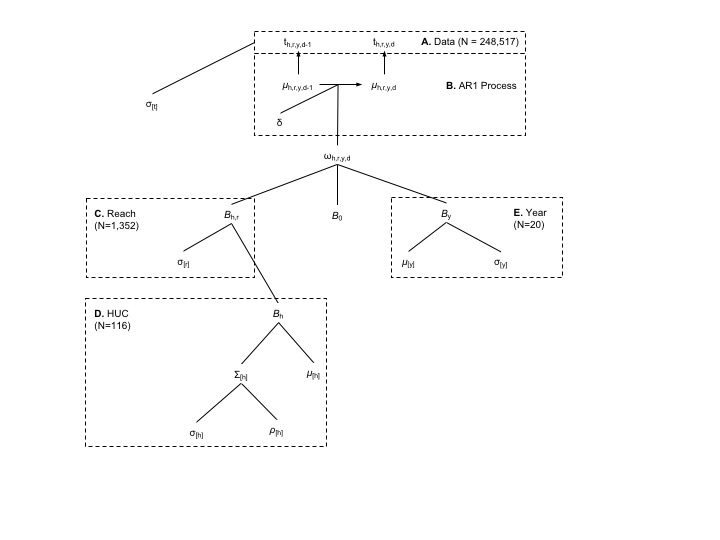
\includegraphics{Figures/Hierarchical_Structure.pdf}
\caption{Hierarchical structure of the daily stream temperature model.
The observed daily temperatures are \(t_{h,r,y,d}\) at HUC8 \(h\) and
reach \(r\) in year \(y\) on day \(d\). In general, \(\mu\) represent
means, \(\sigma\) represent standard deviations, \(B\) represent vectors
of coefficients with subscripts represnting the level of variation,
\(\Sigma\) is the covariance matrix, \(\rho\) is the correlation matrix,
\(\omega\) is the expected temperature as a function of the
deterministic components prior to inclusion of temporal autocorrelation,
and \(\delta\) is the autocorrelation coefficient. See details in the
text for further description of the coefficients.}
\end{figure}

\begin{figure}[htbp]
\centering
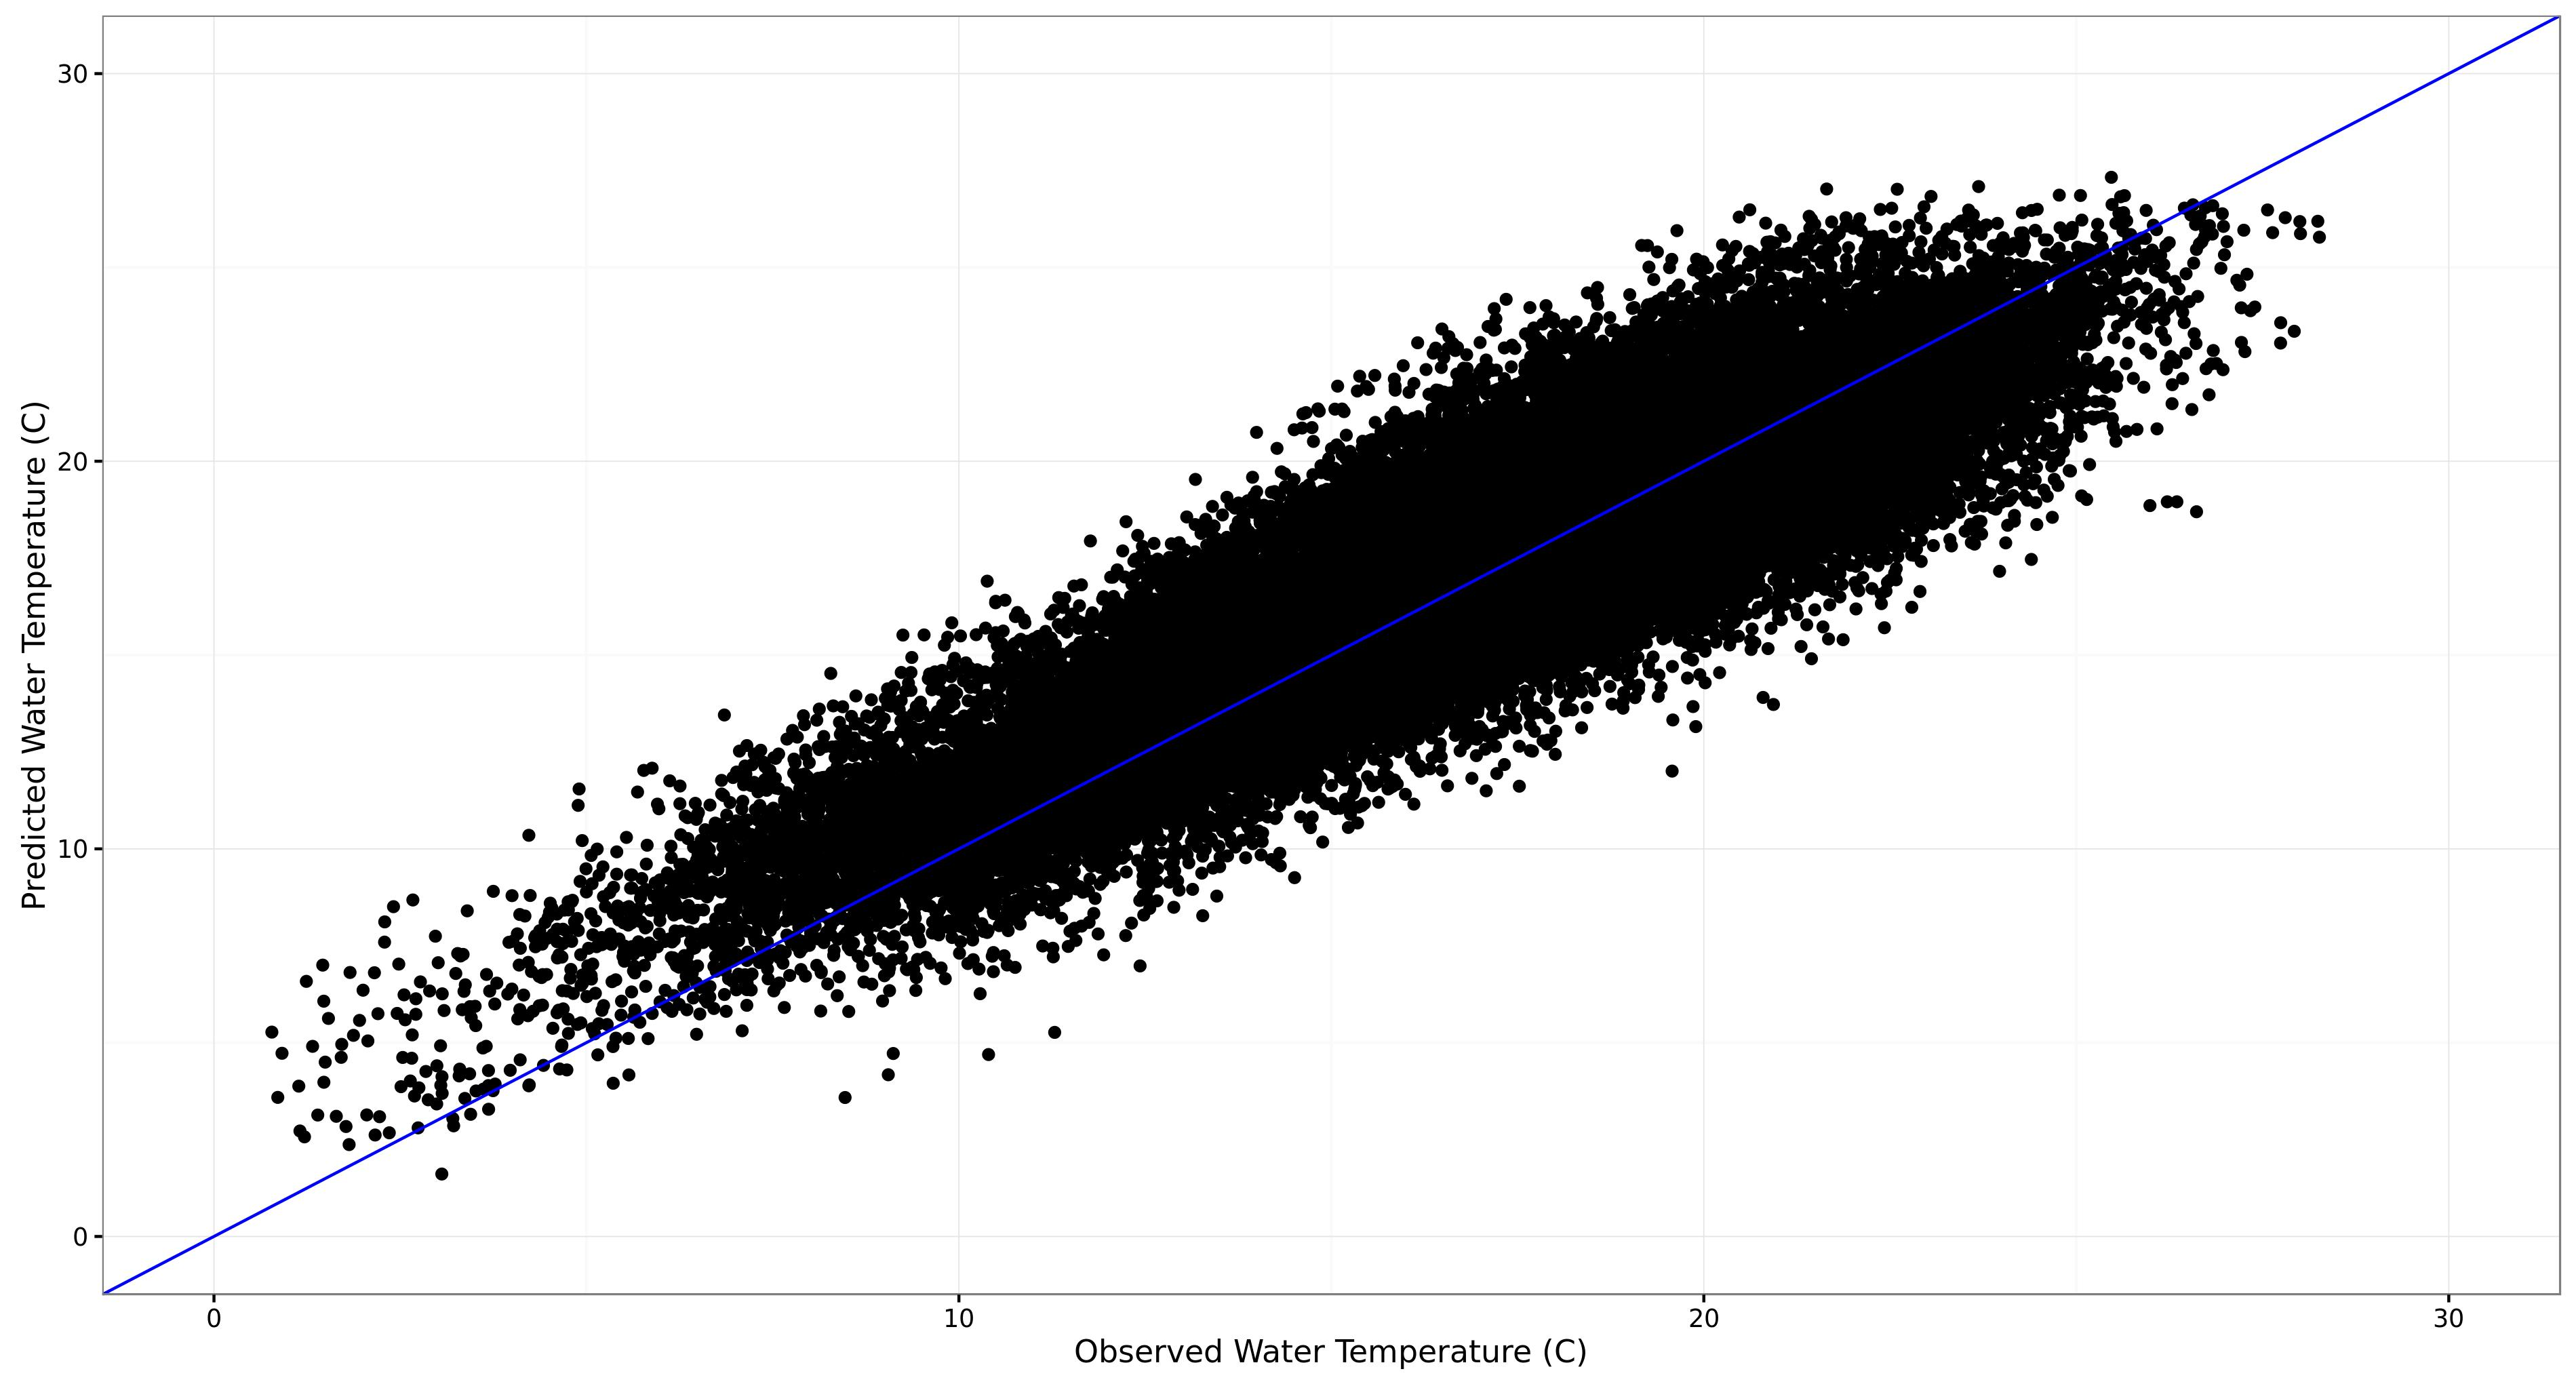
\includegraphics{Figures/validation_plot.jpg}
\caption{trial text}
\end{figure}

\begin{figure}[htbp]
\centering
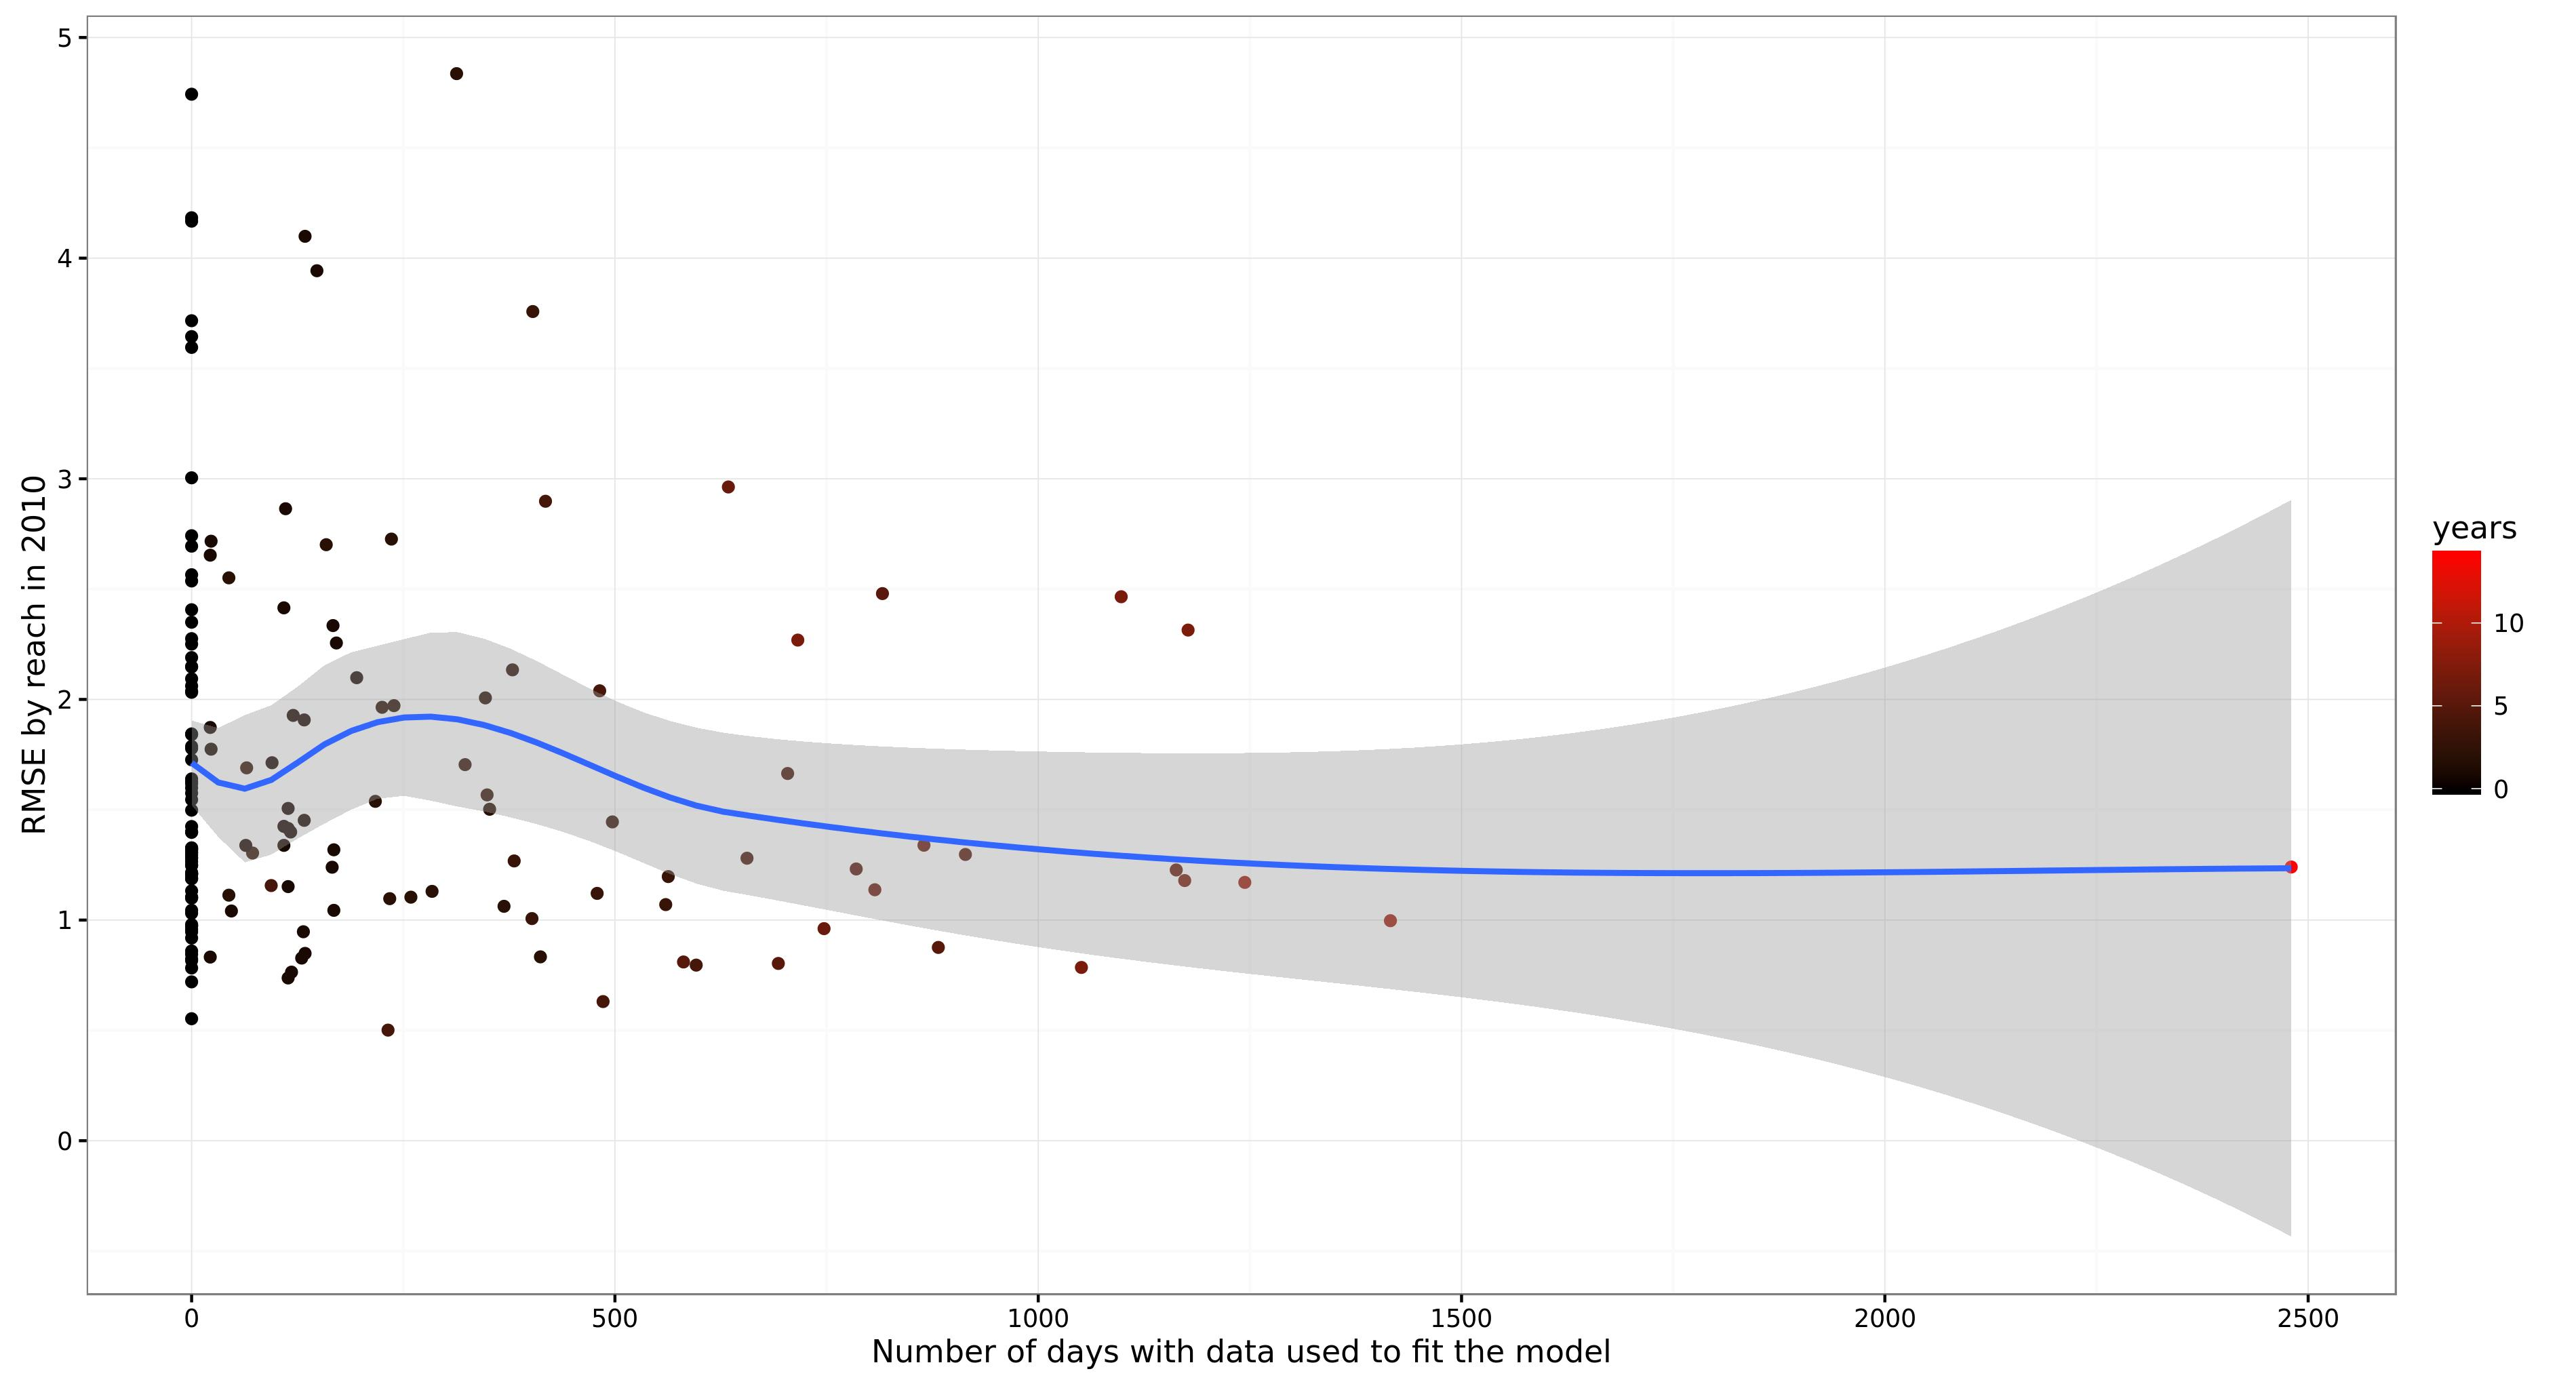
\includegraphics{Figures/rmse_2010_obs_plot.jpg}
\caption{text with \(\sigma=2\) equation}
\end{figure}

\begin{figure}[htbp]
\centering
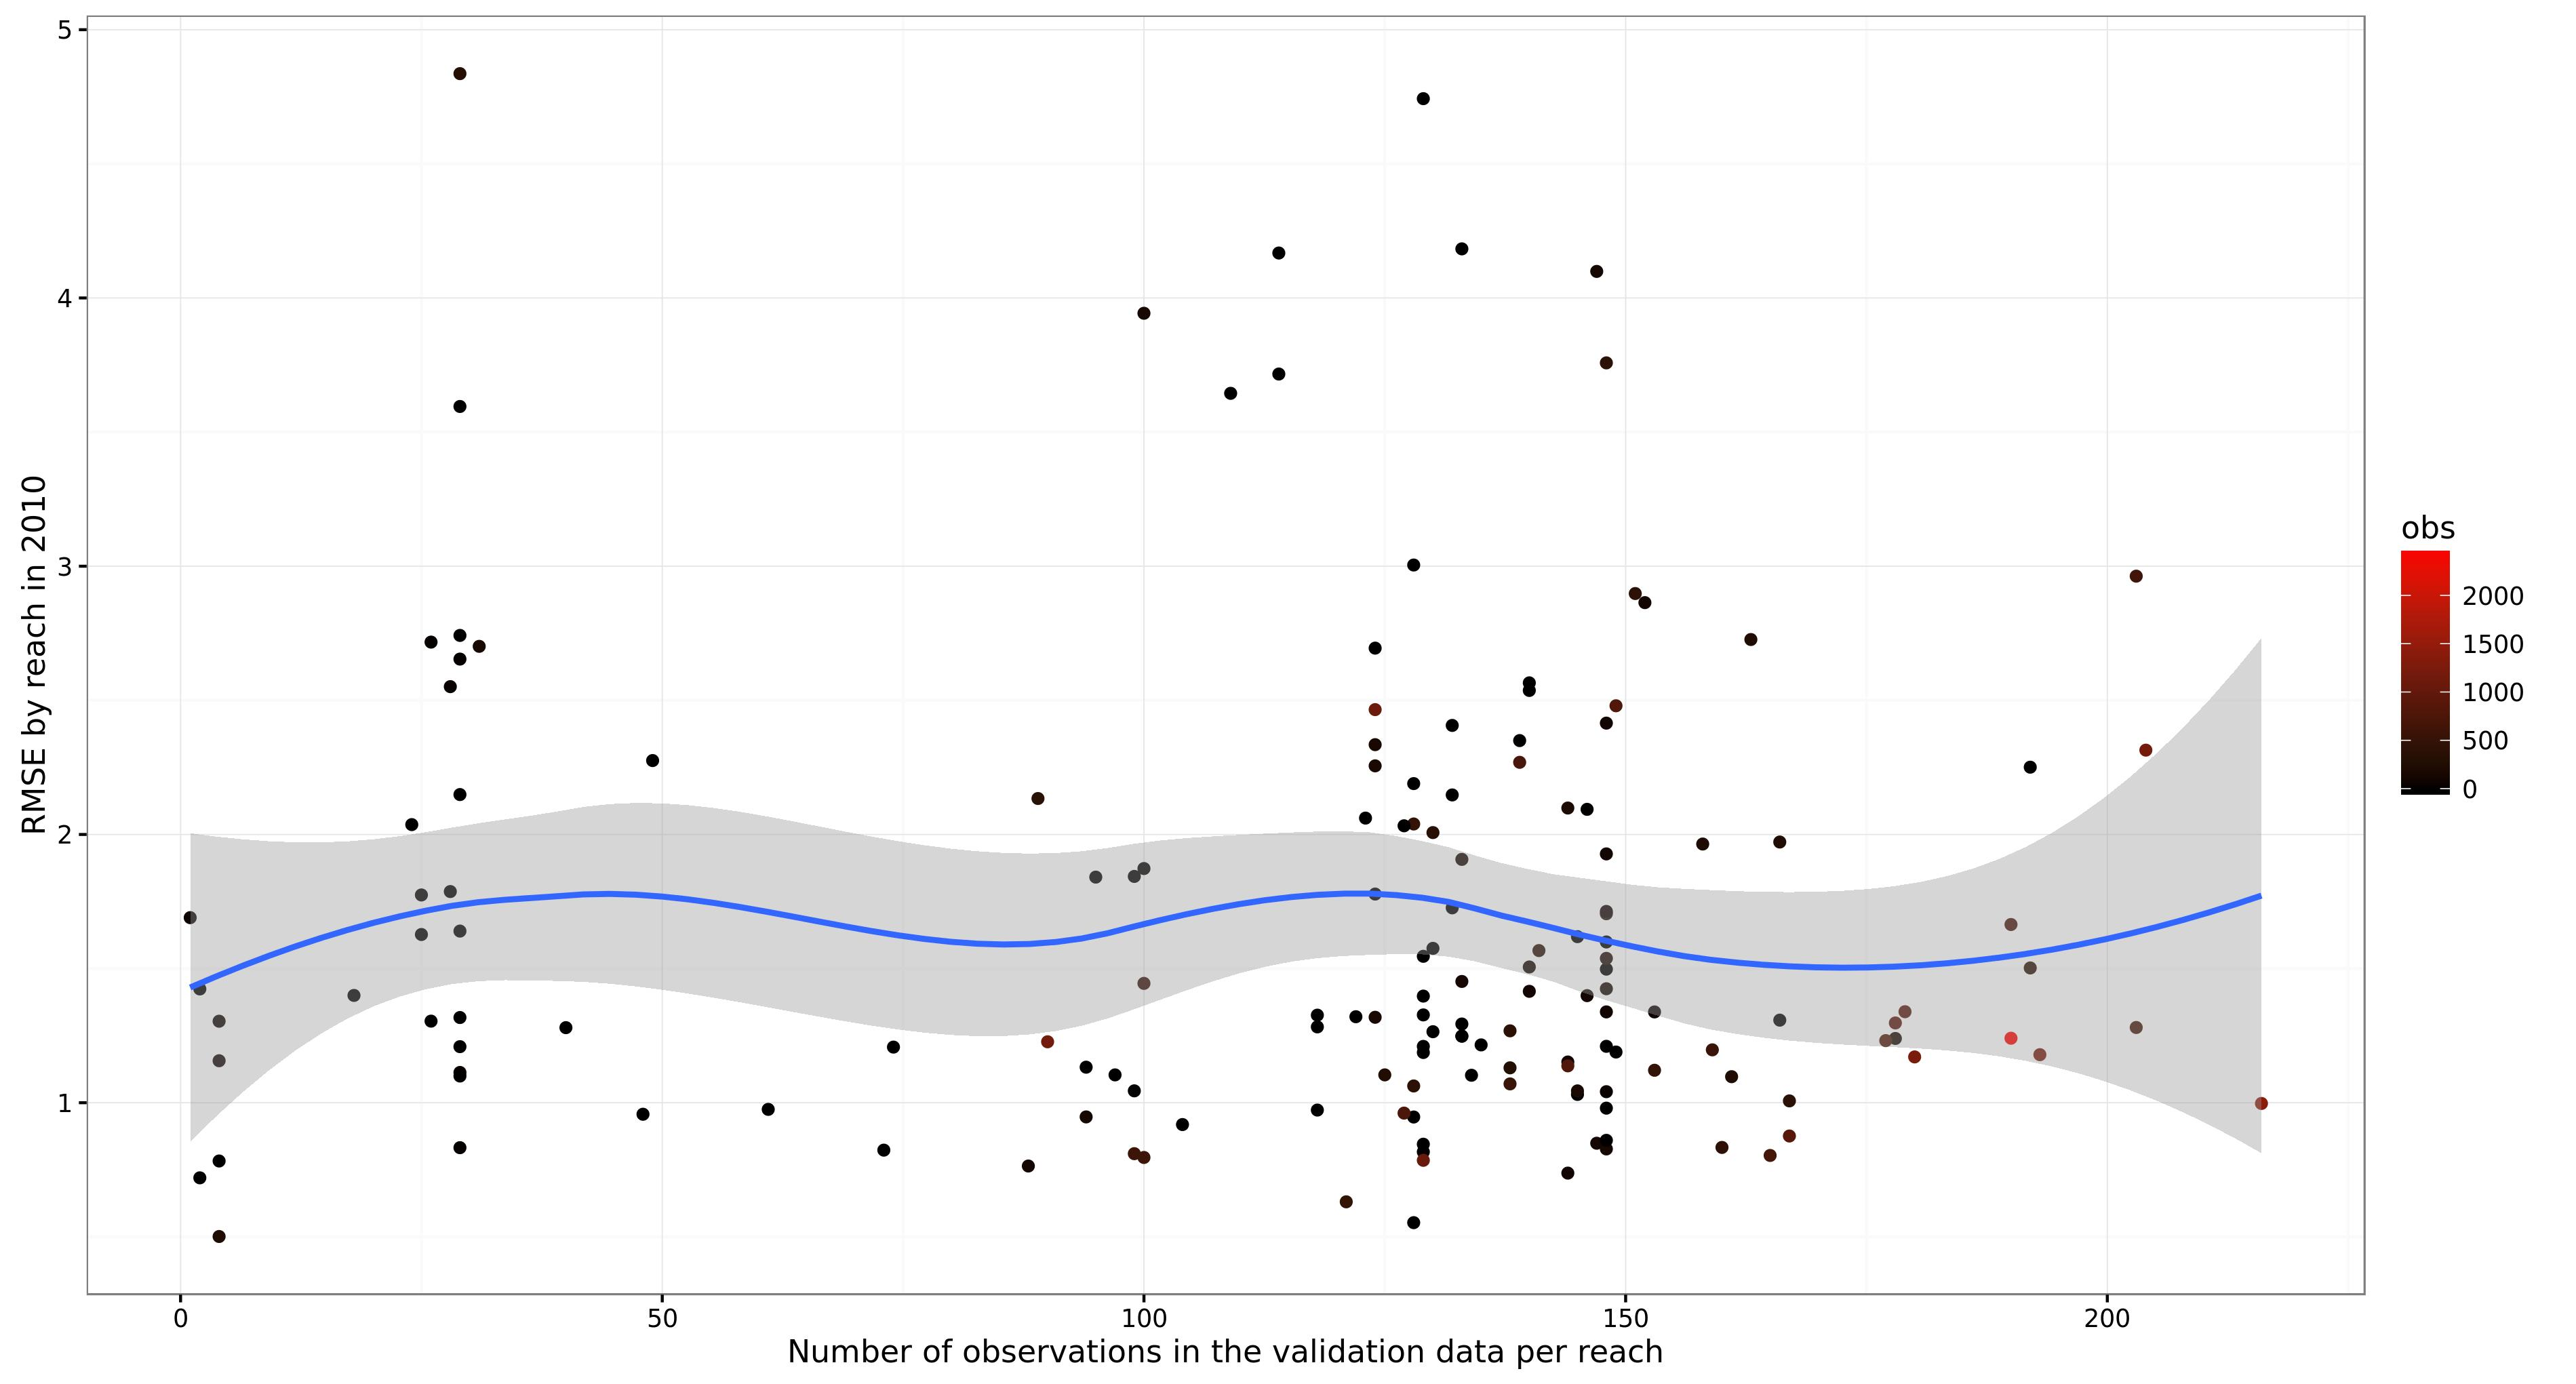
\includegraphics{Figures/rmse_2010_valid_obs_plot.jpg}
\caption{}
\end{figure}

\begin{figure}[htbp]
\centering
\includegraphics{Figures/Inset3.png}
\caption{Figure}
\end{figure}

\begin{figure}[htbp]
\centering
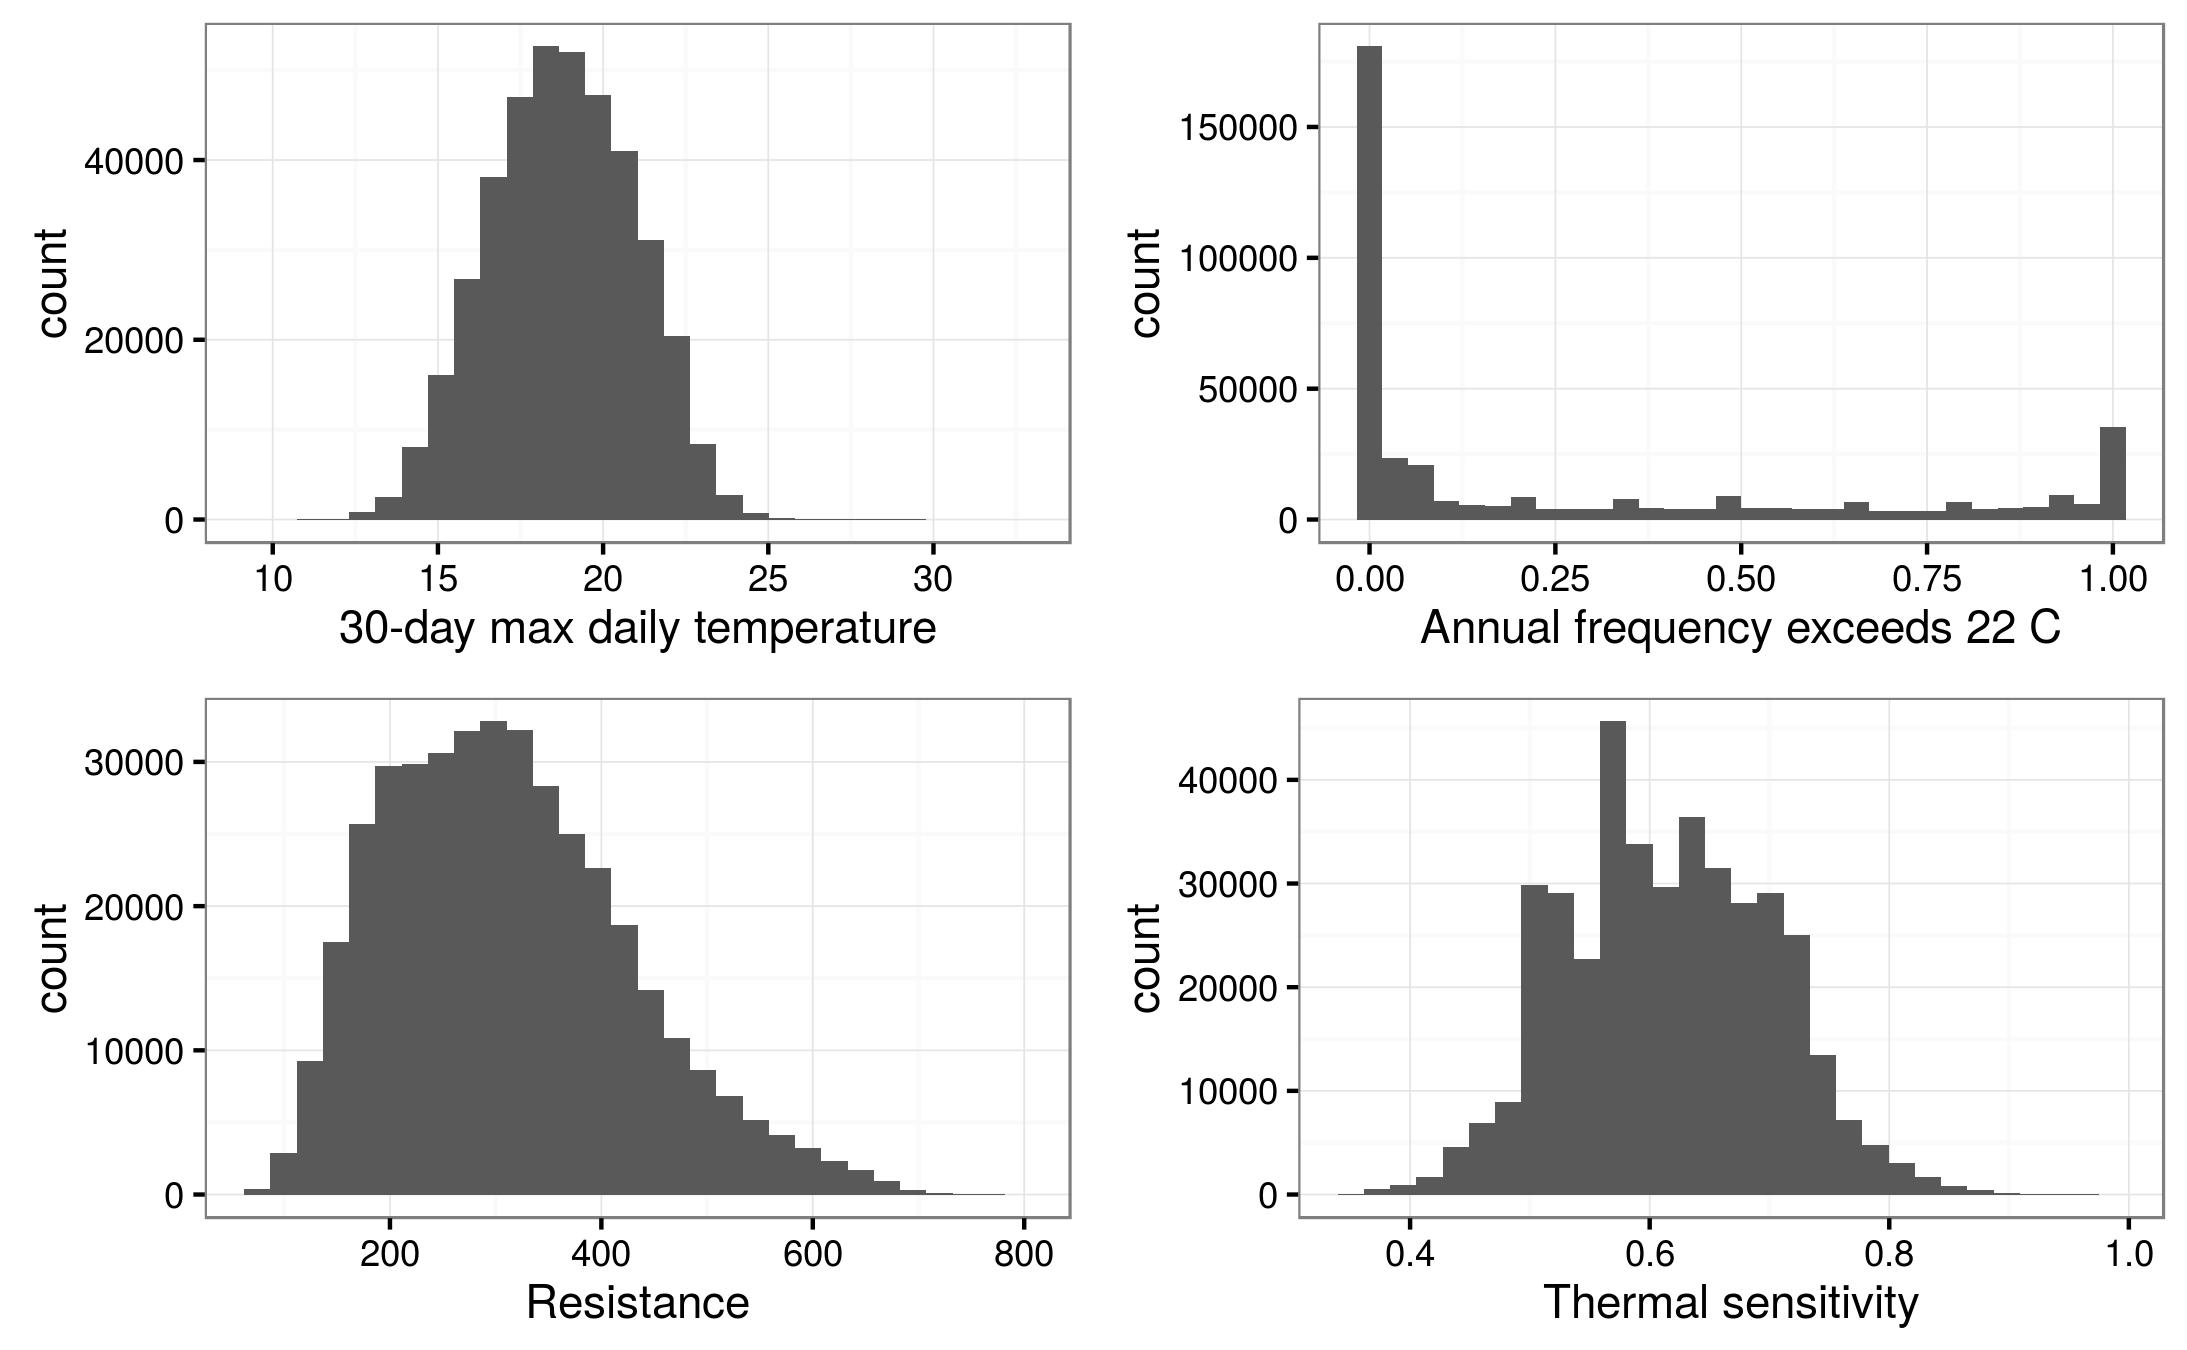
\includegraphics{Figures/metrics_histograms.jpg}
\caption{Figure 6}
\end{figure}

\end{document}
